\usepackage{graphicx}
\section{Difference Image Analysis: Solar System Objects}
\label{sec:dia_solar_system}

\subsection{Difference Image Association}
\label{sec:dia_solar_system_assoc}

So far, difference images have been made only of fields very far from the ecliptic, where solar system objects are expected to be very rare. In particular, the number of known solar system objects in these fields was predicted to be zero: any asteroids actually detected would be new discoveries. Because of this, these fields did not provide a thorough test of known-object association in the difference images: the code ran, but since no known objects were in the field, it found (correctly) that there were zero detections of known objects.

\subsection{Difference Image Linking}
\label{sec:dia_solar_system_link}

These difference images also enabled a test of tracklet creation, the first stage of {\em unknown} asteroid discovery for LSST, using the {\tt make\_tracklets} code. The code was set to require a minimum of 5 sources per tracklet, and run on data sets comprising 10-12 visits, meaning a 5-point tracklet would correspond to an object with a per-image detection probability of only $\sim$50\%. In production, {\tt make\_tracklets} will be set to create tracklets with as few as two sources, but this is viable only in the context of multi-night linking: single-night asteroid discoveries require larger numbers of detections to be confirmed.

So far, {\tt make\_tracklets} has been run on two sets of difference images, one with 10 visits and one with 12.  In the first case, the average number of positive sources per visit (over the 10 visits) was 840; in the second case it was only 430. These numbers are encouragingly low, indicating that Rubin difference images are fairly clean. Accordingly, only nine total tracklets were produced (two in the first run and seven in the second). None of the tracklets had more than the minimum number of 5 detections, and all had inconsistent photometry and a relatively high Great Circle residual (GCR)\footnote{Defined only for tracklets with more than two points, the GCR is the RMS residual relative to the best-fit trajectory that follows a Great Circle on the sky at constant angular velocity. Real asteroids, unless they are very near the Earth, produce tracklets with very low intrinsic GCR: hence, elevated GCR usually indicates a spurious tracklet.}, indicating they were probably spurious. Just as for the known object association, it was unlikely that any unknown asteroids would be found so far from the ecliptic.

Manual examination of image cutouts confirmed the expectation that the tracklet would not correspond to real asteroids: all nine tracklets were entirely composed of spurious sources. This finding of nine spurious tracklets in two fields is not surprising. In production, where two-point tracklets will be generated, thousands of spurious tracklets per visit-pair are expected --- and the downstream multi-night linking softwared based on the HelioLinc3D algorithm is designed to handle this.

More interesting is the nature of the spurious sources that made up the tracklets. All were associated with bright stars. They included diffraction rays, incompletely subtracted scattered light halos, and subtraction residuals near the PSF core. This is very good news, in that all of these types of spurious detections can potentially be eliminated by pre-screening of the source catalogs.

The indications are hopeful that LSST will produce fairly clean difference image source catalogs for input to the asteroid discovery pipeline --- and that pre-screening to make them even cleaner will likely be possible. This is important, because simulations indicate the LSST specifications for the minimum discoverable asteroid (six detections, making up three two-point tracklets, within a two-week time span) are on the edge of what is statistically possible without an unacceptable false-discovery rate. Hence, it is vitally important for the difference image source catalogs to be as clean as possible. Here, at the beginning of commissioning, we are getting our first look at what will be neccessary to achieve this with real LSST data. There's a lot of work to do, but the early indications have us cautiously optimistic.

\section{Single-epoch Image Analysis: Solar System Objects}
\label{sec:sia_solar_system}

\subsection{Single-epoch Linking}
\label{sec:linking}

Prior to the first difference images, we attempted to link asteroids based on source catalogs from the original, un-subtracted images (i.e., calexps). In contrast to the difference image counts averaging 430-840 sources per visit, the average number of sources found on the calexps were 11000, 16000, and 23000 per visit, respectively, on three distinct runs of {\tt make\_tracklets}. The vast majority of these were stars. Nevertheless, because a large number of visits (10--20) had been taken of each field, there was the possiblity that {\tt make\_tracklets} could unambiguously link real asteroids --- especially because some of these fields were relatively near the ecliptic.

The first reasonable test involved ten images taken on November 6. These were engineering images with strong and variable astigmatism caused by testing of bending modes in the mirror support system. Nevertheless, they were sharp enough for the detection of asteroids down to about 23rd magnitude. From an average of 16000 sources per visit, {\tt make\_tracklets} found a total of 3068 tracklets with at least five points. While most of these were unquestionably spurious, nine of them were ten-point tracklets --- that is, each of these nine tracklets corresponded to a distinct object with plausibly asteroidal motion that was detected in {\em every single one} of the ten visits. Moreover, the sources that made up these tracklets showed excellent photometric consistency and relatively low GCR: it was obvious that they were likely to correspond to real asteroids. 

We selected the ten-point tracklet with the very lowest GCR (0.046 arcsec) and checked it against known asteroid ephemerides, obtaining a match to the main belt asteroid \textbf{(193300) 2000 SO275}. This 20th magnitude object is therefore the {\em very first asteroid confirmed to have been detected with the Simonyi Survey Telescope.}

This asteroid has a very well-characterized orbit based on more than 900 observations obtained since its September 2000 discovery. Hence, we could evaluate LSST's astrometric precision by comparing it with predicted positions from JPL. We found the RMS astrometric offset to be 29 milli-arcseconds (mas). To check for a systematic bias, we also calculated the median of the observed-calculated RA and Dec over the ten points, finding 14 mas in RA and 3 mas in Dec --- statistically consistent with zero, as expected.

A timing error could produce a systematic offset in the RA,Dec positions in the direction of motion. To probe this, we evaluted the along-track component of the astrometric offsets, converted it to time via the measured angular velocity, and found a median time offset of 0.3 seconds, which is consistent with zero at the 0.5$\sigma$ level. These excellent astrometric results are especially impressive given the deliberately astigmatic and variable PSF in these engineering images. The telescope has already shown itself to be capable of delivering sharp, round stellar images that will enable even better astrometry.

All of the other ten-point tracklets were found to correspond to known asteroids. So did 12 additional tracklets with only 7--9 points, but with consistent photometry and relatively low GCR --- making 21 real asteroids found by {\tt make\_tracklets} in this single field. This is the same field discussed in Section \ref{sec:association} below, where even more asteroids were found.

\subsection{Single-epoch Association}
\label{sec:association}

Ten images taken in one field on 2024-11-06 and ten each in four fields on 2024-11-23 were close enough to the ecliptic for asteroid association. Around 800 instances of object-source association occurred, identifying around 130 unique objects. Comparing the sources' astrometry to ephemerides, we find very low bias -- the median source is 0.013 arcseconds from its expected position, again indicating that there are not major errors in either timing or astrometry. As for the specific analysis of asteroid (193300) 2000 SO275, these values are statistically consistent with a true systematic error of zero.

\begin{figure}
  \label{fig:solar_system_residuals}
  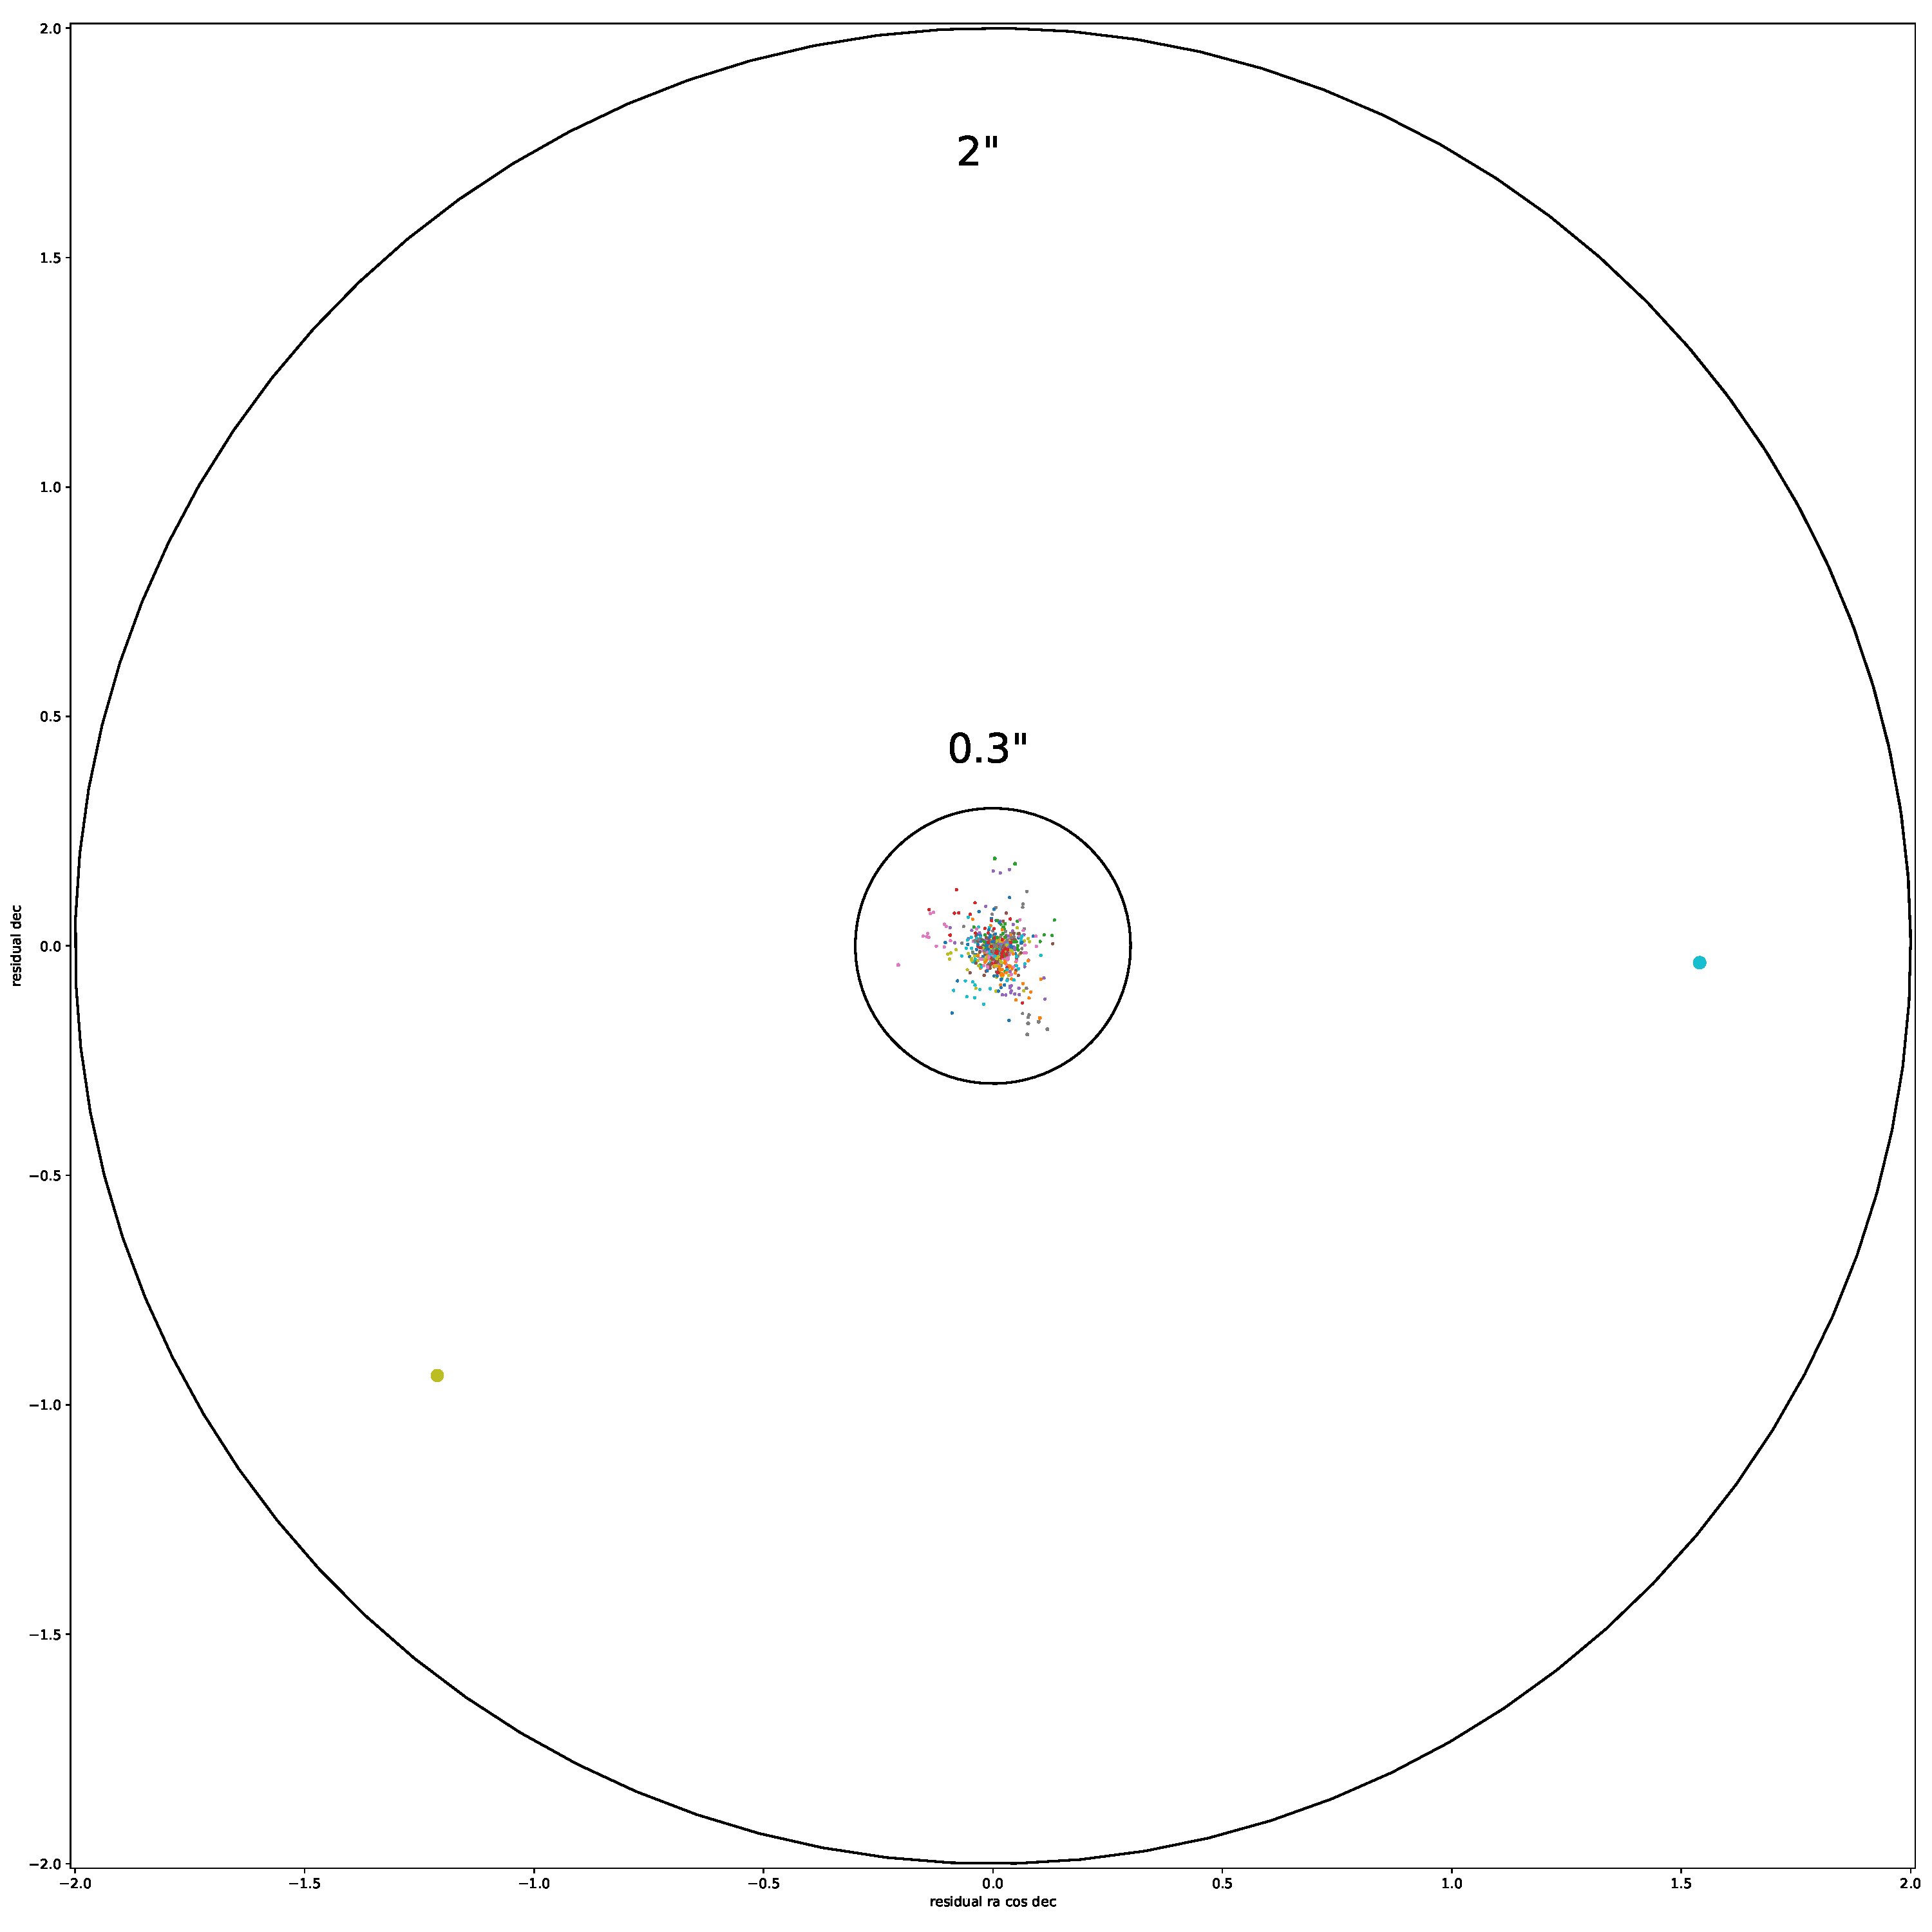
\includegraphics{sso_figures/sso_residuals.pdf}
  \caption{}
\end{figure}
